\documentclass[]{article}
\usepackage{lmodern}
\usepackage{amssymb,amsmath}
\usepackage{ifxetex,ifluatex}
\usepackage{fixltx2e} % provides \textsubscript
\ifnum 0\ifxetex 1\fi\ifluatex 1\fi=0 % if pdftex
  \usepackage[T1]{fontenc}
  \usepackage[utf8]{inputenc}
\else % if luatex or xelatex
  \ifxetex
    \usepackage{mathspec}
  \else
    \usepackage{fontspec}
  \fi
  \defaultfontfeatures{Ligatures=TeX,Scale=MatchLowercase}
\fi
% use upquote if available, for straight quotes in verbatim environments
\IfFileExists{upquote.sty}{\usepackage{upquote}}{}
% use microtype if available
\IfFileExists{microtype.sty}{%
\usepackage{microtype}
\UseMicrotypeSet[protrusion]{basicmath} % disable protrusion for tt fonts
}{}
\usepackage[margin=1in]{geometry}
\usepackage{hyperref}
\PassOptionsToPackage{usenames,dvipsnames}{color} % color is loaded by hyperref
\hypersetup{unicode=true,
            pdftitle={README for the classification tree},
            pdfauthor={Group 2},
            colorlinks=true,
            linkcolor=Maroon,
            citecolor=Blue,
            urlcolor=blue,
            breaklinks=true}
\urlstyle{same}  % don't use monospace font for urls
\usepackage{graphicx,grffile}
\makeatletter
\def\maxwidth{\ifdim\Gin@nat@width>\linewidth\linewidth\else\Gin@nat@width\fi}
\def\maxheight{\ifdim\Gin@nat@height>\textheight\textheight\else\Gin@nat@height\fi}
\makeatother
% Scale images if necessary, so that they will not overflow the page
% margins by default, and it is still possible to overwrite the defaults
% using explicit options in \includegraphics[width, height, ...]{}
\setkeys{Gin}{width=\maxwidth,height=\maxheight,keepaspectratio}
\IfFileExists{parskip.sty}{%
\usepackage{parskip}
}{% else
\setlength{\parindent}{0pt}
\setlength{\parskip}{6pt plus 2pt minus 1pt}
}
\setlength{\emergencystretch}{3em}  % prevent overfull lines
\providecommand{\tightlist}{%
  \setlength{\itemsep}{0pt}\setlength{\parskip}{0pt}}
\setcounter{secnumdepth}{0}
% Redefines (sub)paragraphs to behave more like sections
\ifx\paragraph\undefined\else
\let\oldparagraph\paragraph
\renewcommand{\paragraph}[1]{\oldparagraph{#1}\mbox{}}
\fi
\ifx\subparagraph\undefined\else
\let\oldsubparagraph\subparagraph
\renewcommand{\subparagraph}[1]{\oldsubparagraph{#1}\mbox{}}
\fi

%%% Use protect on footnotes to avoid problems with footnotes in titles
\let\rmarkdownfootnote\footnote%
\def\footnote{\protect\rmarkdownfootnote}

%%% Change title format to be more compact
\usepackage{titling}

% Create subtitle command for use in maketitle
\providecommand{\subtitle}[1]{
  \posttitle{
    \begin{center}\large#1\end{center}
    }
}

\setlength{\droptitle}{-2em}

  \title{README for the classification tree}
    \pretitle{\vspace{\droptitle}\centering\huge}
  \posttitle{\par}
    \author{Group 2}
    \preauthor{\centering\large\emph}
  \postauthor{\par}
      \predate{\centering\large\emph}
  \postdate{\par}
    \date{\texttt{December,\ 2nd,\ 2019}}


\begin{document}
\maketitle
\begin{abstract}
This Chapter is describes the classification tree algorithm applied to
the CleanClass2007to2014\_2 data coded in the script
`ClassificationTree.R'.
\end{abstract}

\hypertarget{fundamentals-of-classification-trees}{%
\subsection{Fundamentals of Classification
Trees}\label{fundamentals-of-classification-trees}}

Classification trees split the different variables in order to obtain
the most homogeneos possible clusters, by minimizing a loss function,
that can be restricted (this complexity parameter is called cp in the
rpart-Package). For every split it computes the sum of the errors on
both sides of the split for all Variables and chooses the one with the
lowest error.

\hypertarget{our-approach}{%
\subsection{Our Approach}\label{our-approach}}

As also applied in the other models, we use all the available
information just before the 2014 NFL-Draft, in order to train the model
and then apply it on the data for 2014. In other words we act as if it
was the end of April 2014 (which is one week before the draft).

For growing trees on our College League / NFL Draft data, we check
whether the best results can be optained, by manually splitting the data
sets on the three postitions (QB / WR / RB) or if the computer will do
that on his own. For growing the trees we use the rpart-Package, which
is commonly used for this purpose, since it does very much on his own.
When growing a tree it uses k-fold cross-validation (by default k=10)
for optimizing the model with respect to the best complexity and the
spots to split. Therefore we do no further cross-validation on the data
set.

Here you can see the different trees, that we grew, plotted with the
fancyRpartPlot-function out of the rattle-Package. Since we use data
with many variables and a couple of splits are made, the plots are not
really readable. The aim of showing them, is to visualize the complexity
of the trees.

\begin{figure}
\centering
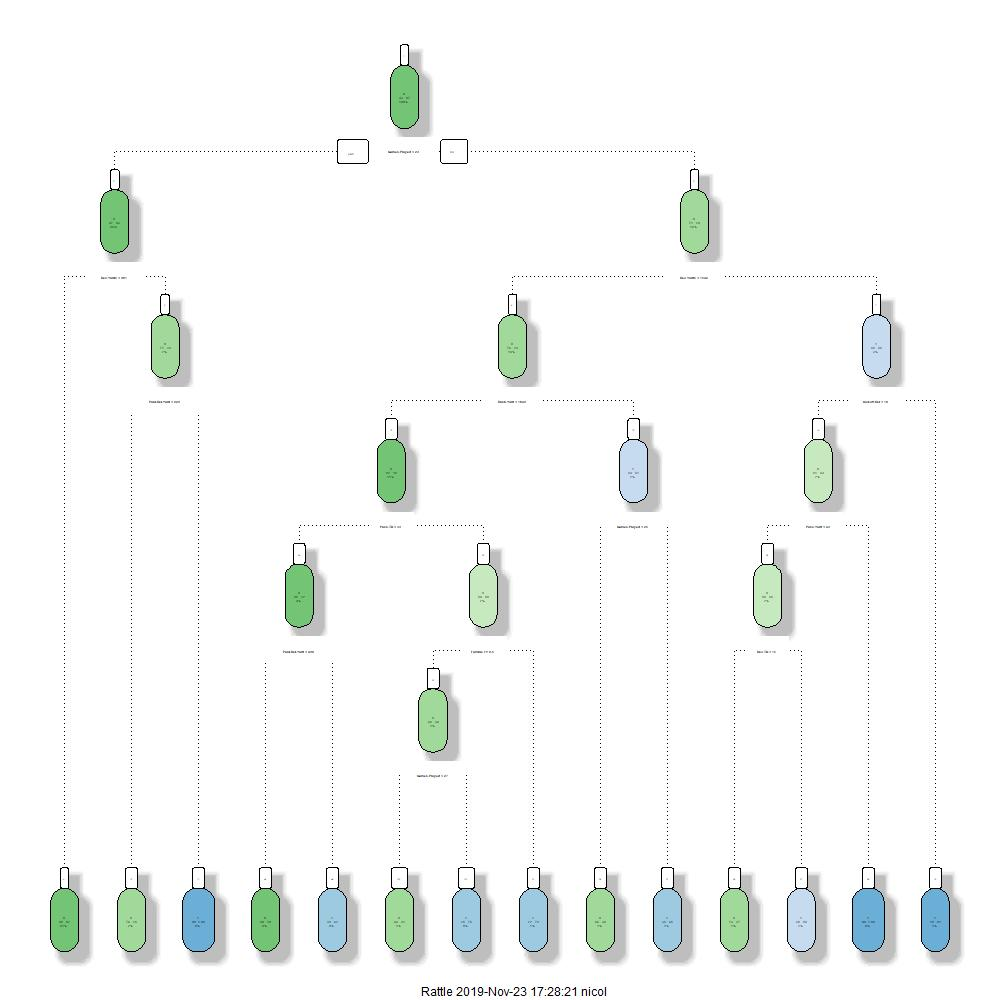
\includegraphics{../../Project_Scripts/Togtree.jpg}
\caption{Classification Tree for the whole data}
\end{figure}


\end{document}
